\documentclass{../../presentation}

\title{PSE - Vorkurs Tag 1}
\author{Linus, Philipp, Tillmann, Tobias}
\institute{FIUS - Fachgruppe Informatik Universität Stuttgart}
\date{06.09.2025}

\makeatletter
\renewcommand{\lecture@pathprefix}[1]{../../logos/}
\makeatother

\usepackage{todonotes}
\setuptodonotes{inline}

\begin{document}

\begin{frame}
  \titlepage
\end{frame}

\begin{frame}
  \listoftodos
\end{frame}

\section{Introduction}

\begin{frame}
  \todo{Neu machen kommt auf aufgaben Blatt}
\end{frame}

\begin{frame}[fragile]
  \frametitle{WLAN}
  Die Universität bietet ein Gast WLAN an jedoch wollen wir in das offizielle WLAN der Universität einsteigen.
  \newline
  \begin{itemize}
    \item iOS und Android
    \item Windows
    \item MacOS
    \item Linux
  \end{itemize}
\end{frame}

\begin{frame}[fragile]
  \frametitle{WLAN - iOS und Android}
  \begin{itemize}
    \item Im AppStore bzw. Playstore nach \enquote{geteduroam} suchen und die App installieren
    \item Dann nach Universität Stuttgart suchen
    \item Nun Student wählen und eure Daten eingeben
    \item \texttt{stxxxxxx@stud.uni-stuttgart.de} - Benutzername
    \item Und eurer Passwort eingeben
    \item Nun auf Verbinden klicken und fertig
  \end{itemize}
\end{frame}

\begin{frame}[fragile]
  \frametitle{WLAN - Windows}
  \begin{itemize}
    \item Im Internet auf \href{https://geteduroam.app}{\enquote{geteduroam.app}} gehen und die Windows Version herunterladen
    \item Dann nach Universität Stuttgart suchen
    \item Nun Student wählen und eure Daten eingeben
    \item Nun auf Verbinden klicken und fertig
  \end{itemize}
\end{frame}

\begin{frame}[fragile]
  \frametitle{WLAN - MacOS}
  \begin{itemize}
    \item Im Internet auf \href{http://uni-stuttgart.de/eduroam}{\enquote{uni-stuttgart.de/eduroam}} gehen
    \item und als Gruppe \enquote{Student} wählen
    \item Lädet das Konfigurationspaket herunter
    \item In euren Systemeinstellungen auf \enquote{Geräteverwaltung} gehen
    \item Nun über das Plus-Symbol das Konfigurationspaket hinzufügen
    \item \texttt{stxxxxx} - Benutzername
    \item Und euer Passwort eingeben
    \item Nun auf Verbinden klicken und fertig
  \end{itemize}
\end{frame}

\begin{frame}[fragile]
  \frametitle{WLAN - Linux}
  \begin{itemize}
    \item Im Internet auf \href{http://uni-stuttgart.de/eduroam}{\enquote{uni-stuttgart.de/eduroam}} gehen
    \item Als Benutzergruppe \enquote{Student} wählen
    \item Unten links auf \enquote{einen anderen Installer auswählen} klicken
    \item \enquote{Linux} auswählen
    \item Über den Button das Pythonskript herunterladen
    \item Im Terminal mit \texttt{\$ python3 [Dateipfad zum Pythonskript]} ausführen
    \item Den Anweisungen folgen und Benutzername (\texttt{stxxxxxx@stud.uni-stuttgart.de}) sowie Passwort eingeben
  \end{itemize}
\end{frame}

\begin{frame}
  \frametitle{IntelliJ IDEA}
  \textbf{\achtung{} Wir werden uns Lediglich auf IntelliJ IDEA konzentrieren, wenn ihr eine andere IDE nutzen wollt, können wir keinen Support garantieren. }
  \newline
  \begin{itemize}
    \item Wir laden uns erst die JetBrains Toolbox herunter, um die IDE zu installieren
    \item Dann installieren wir IntelliJ IDEA Community Edition
  \end{itemize}
\end{frame}

\begin{frame}
  
\includegraphics[width=1\linewidth]{img/memeIDE.jpg}
\end{frame}

\begin{frame}
  \frametitle{IntelliJ IDEA - Installation}
  \begin{tikzpicture}[remember picture,overlay]
    \node[at=(current page.center), anchor=center, yshift=-2] {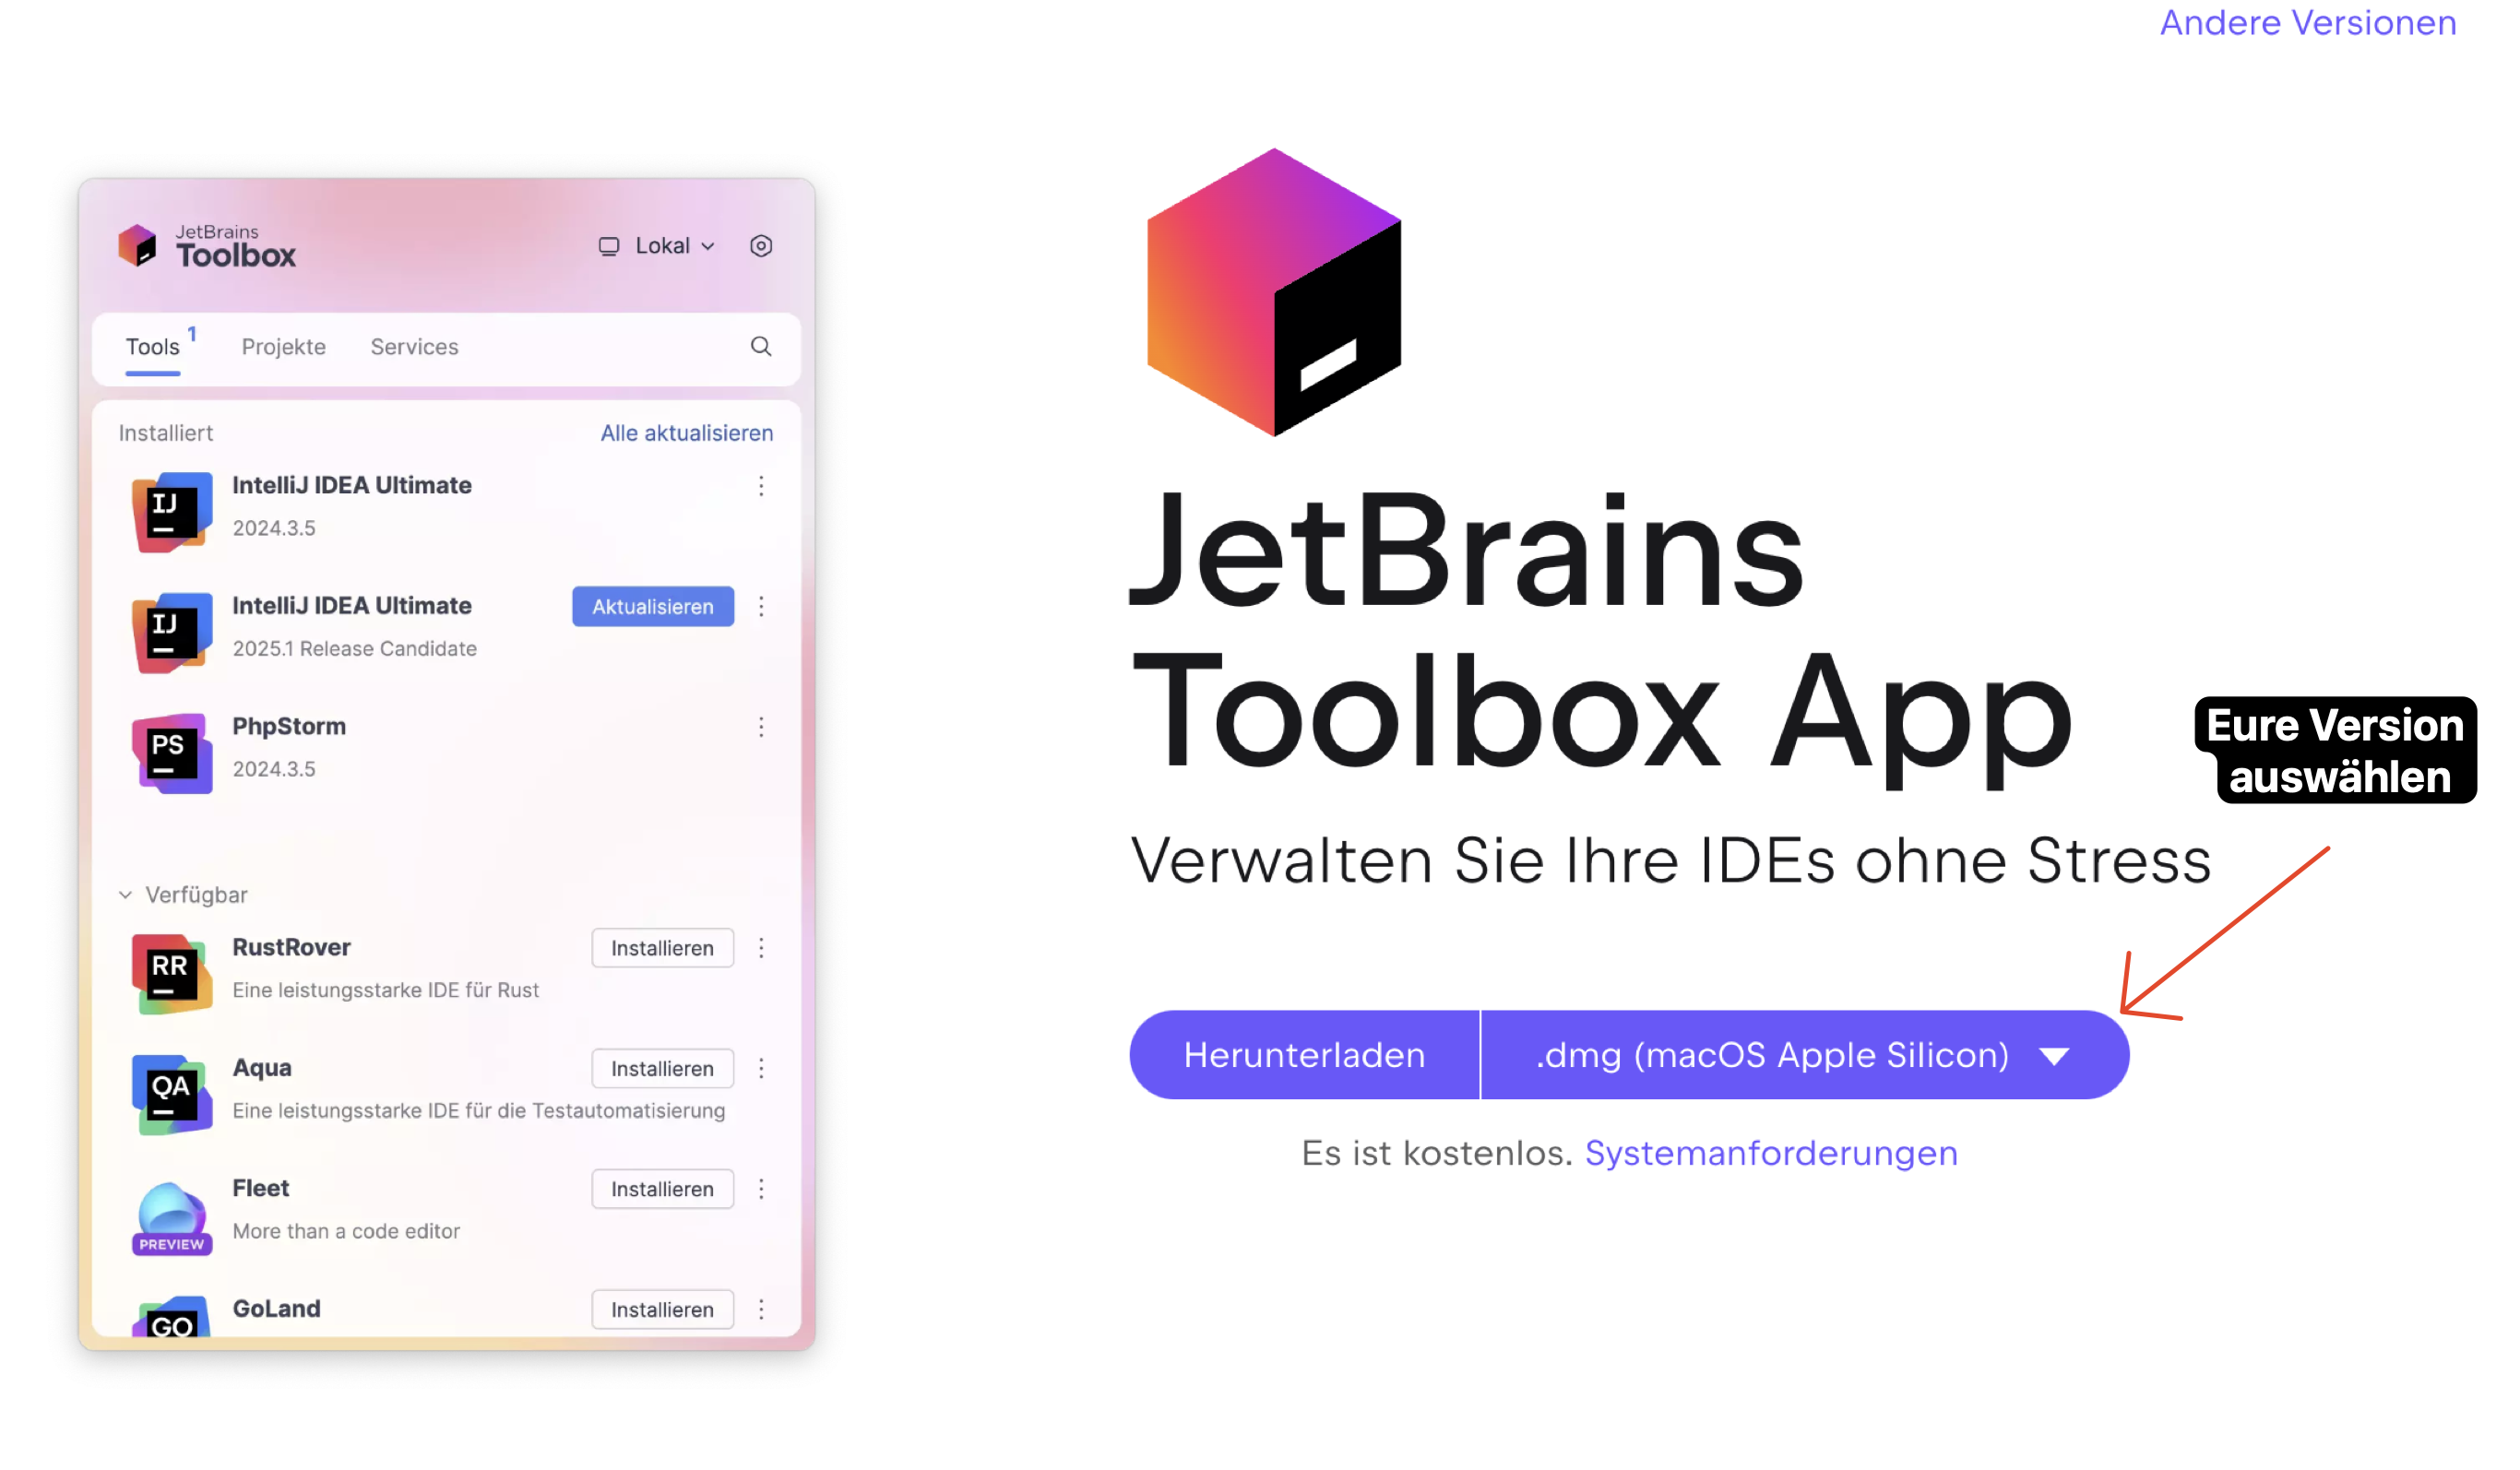
\includegraphics[width=1\linewidth]{img/toolBoxDownload.png}};
    \node[at=(current page.north), anchor=north, align=center, yshift=-1.2cm] {Geht auf \href{https://www.jetbrains.com/de-de/toolbox-app/}{\texttt{\enquote{jetbrains.com/toolbox-app/}}} und ladet die Toolbox herunter.};
  \end{tikzpicture}
\end{frame}

\begin{frame}
  \frametitle{IntelliJ IDEA - Installation}
  \begin{tikzpicture}[remember picture,overlay]
    \node[at=(current page.east), anchor=east, yshift=-2] {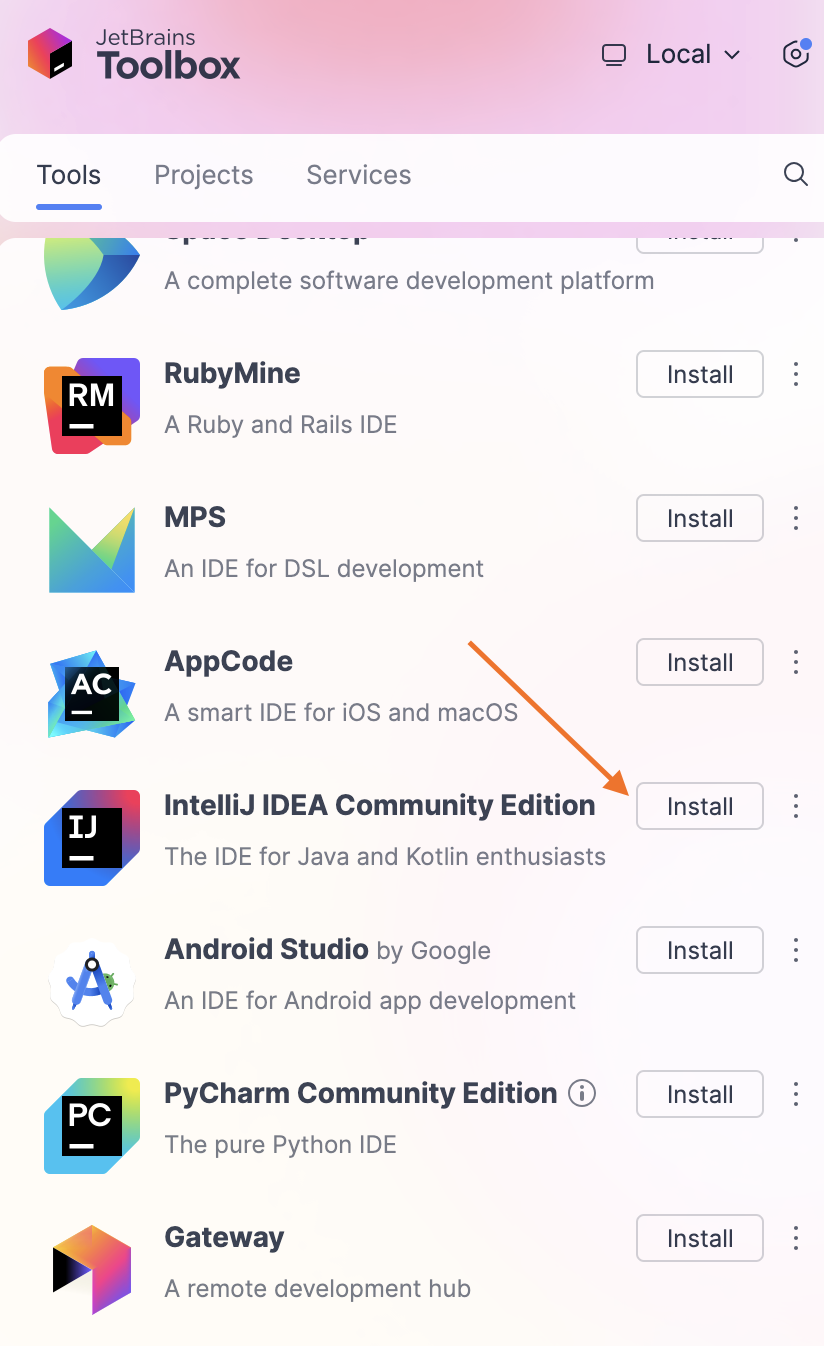
\includegraphics[width=.35\linewidth]{img/IntelliJDownload.png}};
    \node[at=(current page.west), anchor=west, align=center, yshift=0cm, xshift=2cm, text width=8cm] {Nach der Installation der Toolbox öffnet sich ein Fenster, in dem ihr die IDE auswählen könnt, die ihr installieren wollt. Wählt \enquote{IntelliJ IDEA Community Edition} aus und klickt auf \enquote{Install}. \newline \todo{Besser machen}};
  \end{tikzpicture}
\end{frame}

\begin{frame}
  \frametitle{JDK - Installation}
  Wir benötigen ein JDK (Java Development Kit), um Java Programme zu schreiben und auszuführen.
  \newline
  \begin{itemize}
    \item \achtung{} MacOS: auf File/ Datei gehen oben links in der Menüleiste
    \item Nun auf \texttt{Project Structure} klicken
    \item Dann auf \texttt{SDKs} klicken
    \item Dann auf das Plus-Symbol klicken und auf \texttt{Download JDK} klicken
  \end{itemize}
\end{frame}

\begin{frame}
  \frametitle{JDK - Installation}
  \achtung{} Die Universität nutzt die OpenJDK Version 21, die wir auch verwenden werden.
  \begin{itemize}
    \item Dann Microsoft OpenJDK als Anbieter/ Vendor auswählen
    \item Und nen geeigneten Speicher Ort auswählen, der Standart Pfad sollte aber ausreichen.
  \end{itemize}
\end{frame}

\begin{frame}
  \frametitle{Projekt erstellen}
  \begin{itemize}
    \item In IntelliJ auf neues Projekt erstellen/ New Project klicken
    \item Java auswählen und das Projekt firstProjekt nennen
    \item Nun nen geeigneten Speicher Ort auswählen \achtung{} KEIN Git Reposotory erstellen
    \item Als Build System IntelliJ verwenden und als JDK unsere derzeitig herruntergeladene 21 auswählen
    \item Wir wollen keinen Sample Code
  \end{itemize}
\end{frame}

\begin{frame}
  \frametitle{Projekt erstellen}
  Es sollte nun so bei euch aussehen:

  \vspace{1cm}

  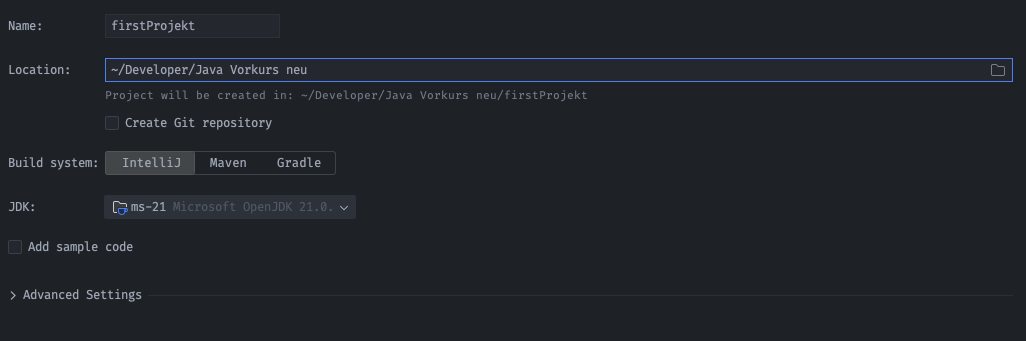
\includegraphics[width=1\linewidth]{img/projektCreation.png}
\end{frame}

\begin{frame}
  \frametitle{Projekt erstellen}
  \begin{itemize}
    \item Nun auf \texttt{Create} klicken und das Projekt wird erstellt
    \item Nun links in der Projektansicht auf \texttt{src} rechtsklicken und eine neue Java Klasse erstellen
    \item Diese Klasse \texttt{Main} nennen und auf \texttt{Enter} drücken
    \item Nun sollte sich eine neue Datei öffnen, in der wir unseren Code schreiben
  \end{itemize}
\end{frame}

\begin{frame}[fragile]
  \frametitle{Erste Java Klasse}
  Nun schreiben wir folgenen Code in die Main Klasse rein
  \begin{minted}{java}
    public class Main {
      public static void main(String[] args) {
        System.out.println("Hallo Welt!");
      }
    }
  \end{minted}
  \achtung{} Was das alles bedeutet werden wir euch dann in den nächsten Tagen erklären!
\end{frame}

\begin{frame}
  \frametitle{Erste Java Klasse}
  \begin{itemize}
    \item Das Programm soll nun bei allen von euch gestartet werden
    \item Dazu klickt auf das grüne Dreieck oben rechts in der IDE
    \item Wenn alles korrekt eingerichtet ist, sollte die Ausgabe "Hallo Welt!" erscheinen.
          \achtung{} Wenn eine Fehlermeldung erscheint, überprüft bitte den Code ansonsten fragt einen Tutor.
  \end{itemize}
\end{frame}

\begin{frame}
  \frametitle{GitHub}
  GitHub ist eine Plattform, auf der man Code online speichern, verwalten und mit anderen teilen kann. Es basiert auf Git, einem Versionskontrollsystem.
\end{frame}

\begin{frame}
  \frametitle{Warum GitHub für Java-Projekte?}
  \pause
  \begin{itemize}
    \item \textbf{Sicherung:} Java-Code (Klassen, Methoden, Projekte) kann sicher gespeichert werden.
          \pause
    \item \textbf{Versionskontrolle:} Änderungen zwischen Versionen sind nachvollziehbar – praktisch beim Lernen oder bei Fehlern.
          \pause
    \item \textbf{Zusammenarbeit:} Gemeinsames Arbeiten an Projekten und Feedback sind möglich.
          \pause
    \item \textbf{Überall verfügbar:} Zugriff von verschiedenen Orten – beispielsweise an der Uni, zuhause oder unterwegs.
  \end{itemize}
\end{frame}

\begin{frame}[fragile]
  \frametitle{Variablen}
  \pause
  \begin{itemize}
    \item Variablen werden benötigt, um Werte im Programm zwischenzuspeichern
    \item Variablen haben einen Namen (Bezeichner), einen Datentyp und speichern einen Wert
    \item Über den Namen kann später auf den gespeicherten Wert zugegriffen werden
          \pause
          \begin{minted}{java}
      int alter = 20;
    \end{minted}
    \item Hier ist \texttt{alter} der Name der Variable, \texttt{int} der Datentyp (ganzzahlige Zahl) und \texttt{20} der gespeicherte Wert
  \end{itemize}
\end{frame}

\begin{frame}[fragile]
  \frametitle{Konzept Null}
  \pause
  \begin{itemize}
    \item \texttt{null} steht für „kein Wert“
          \begin{minted}{java}
      String name = null; // name zeigt auf nichts
      \end{minted}
          \pause
    \item Zugriff auf Methoden oder Eigenschaften einer \texttt{null}-Referenz führt zu einem Fehler (\color{red}\texttt{NullPointerException}).
  \end{itemize}
  \pause
  \achtung{} \texttt{null} ist nicht dasselbe wie eine leere Zeichenkette (\texttt{""}) oder die Zahl 0.
\end{frame}

\begin{frame}[fragile]
  \frametitle{Variablen}
  \pause
  \begin{itemize}
    \item Deklaration \quad \textrightarrow \quad Variable wird erstellt \textbf{OHNE} einen Wert zuzuweisen
          \begin{minted}{java}
      int zahl;
    \end{minted}
          \pause
    \item Initialisierung \quad \textrightarrow \quad Variable wird sein \textbf{ERSTER} Wert zugewiesen
          \begin{minted}{java}
      zahl = 42;
    \end{minted}
          \pause
  \end{itemize}
  \begin{minted}{java}
  //In der Regel Deklaration und Initialisierung gleichzeitig
  int zahl = 42;

  //aber auch so möglich
  int zahl;
  // ...
  zahl = 42;
  \end{minted}
\end{frame}

\begin{frame}[fragile]
  \frametitle{Variablen}
  \pause
  \begin{itemize}
    \item Variablen können auch später im Programm verändert werden
          \begin{minted}{java}
      int alter = 20;
      alter = 21; // alter ist jetzt 21
    \end{minted}
  \end{itemize}
\end{frame}

\begin{frame}
  \frametitle{Datentypen in Java}
  \pause
  \centering
  \rowcolors{2}{tablerow}{white}
  \begin{tabular}{l l}
    \rowcolor{tablehead}
    \textbf{Typ} & \textbf{Beschreibung}                          \\
    int          & Ganzzahlen (z.\,B. 1, 2, 3)                    \\
    float        & Kommazahlen (weniger genau)                    \\
    double       & Kommazahlen (hohe Genauigkeit)                 \\
    char         & Einzelnes Zeichen (z.\,B. 'a')                 \\
    short        & Kleine Ganzzahlen                              \\
    long         & Große Ganzzahlen                               \\
    boolean      & Wahrheitswert (\texttt{true} / \texttt{false}) \\
    String       & Text (z.\,B. "Hallo")                          \\
  \end{tabular}
\end{frame}


\begin{frame}
  \frametitle{Operatoren in Java}
  \pause
  \centering
  \rowcolors{2}{tablerow}{white}
  \begin{tabular}{l l l}
    \rowcolor{tablehead}
    \textbf{Operator} & \textbf{Bedeutung}    & \textbf{Gültige Typen} \\
    +                 & Addition / Verkettung & Zahlen, String         \\
    -                 & Subtraktion           & Zahlen                 \\
    *                 & Multiplikation        & Zahlen                 \\
    /                 & Division              & Zahlen                 \\
    \%                & Modulo (Rest)         & Ganzzahlen             \\
  \end{tabular}
\end{frame}

\begin{frame}[fragile]
  \frametitle{Beispiel: String + Zahl}
  \pause
  \begin{minted}{java}
String text = "Ergebnis: ";
int zahl = 5;
System.out.println(text + zahl);
  \end{minted}
  \pause
  \begin{ausgabe}
    Ergebnis: 5
  \end{ausgabe}
\end{frame}

\begin{frame}[fragile]
  \frametitle{Kommentare in Java}
  \pause
  \begin{itemize}
    \item \texttt{// Einzeilige Kommentare}
    \item \texttt{/* Mehrzeilige Kommentare */}
  \end{itemize}
  \pause
  \vspace{1em}
  \begin{minted}{java}
float gewicht = 23.4; // Gewicht in kg

/*
Berechnet die Summe
zweier Zahlen
*/
int summe = x + y;
  \end{minted}
\end{frame}

\begin{frame}[fragile]
  \frametitle{Textausgabe in Java}
  \pause
  Problem: Wir wollen irgendwas in der Konsole ausgeben
  \pause
  \vspace{0.5em}
  \begin{minted}{java}
System.out.print("Das ist eine Konsolen Ausgabe");
  \end{minted}
  \begin{ausgabe}
    Das ist eine Konsolen Ausgabe
  \end{ausgabe}
  \pause
  \begin{minted}{java}
System.out.print("Das ist eine Konsolen Ausgabe");
System.out.print("Das ist noch eine Ausgabe");
  \end{minted}
  \pause
  \begin{ausgabe}
    Das ist eine Konsolen AusgabeDas ist noch eine Ausgabe
  \end{ausgabe}
\end{frame}

\begin{frame}[fragile]
  \frametitle{Zeilenumbruch: println und \textbackslash n}
  \pause
  \begin{minted}{java}
System.out.println("1. Ausgabe");
System.out.println("2. Ausgabe");
  \end{minted}
  \pause
  \begin{ausgabe}
    1. Ausgabe \newline
    2. Ausgabe
  \end{ausgabe}
  \pause
  \begin{minted}{java}
System.out.print("1. Ausgabe\n");
System.out.print("2. Ausgabe");
  \end{minted}
  \pause
  \begin{ausgabe}
    1. Ausgabe \newline
    2. Ausgabe
  \end{ausgabe}
\end{frame}

\begin{frame}[fragile]
  \frametitle{Ausgabe von Variablen}
  \pause
  Man kann nicht nur Text, sondern auch Variablen ausgeben:
  \pause
  \begin{minted}{java}
int number = 42;
System.out.println(number);
  \end{minted}
  \begin{ausgabe}
    42
  \end{ausgabe}
  \pause
  Oder beides kombiniert:
  \begin{minted}{java}
int number = 42;
System.out.println("Meine Lieblingszahl ist " + number + "!");
  \end{minted}
  \pause
  \begin{ausgabe}
    Meine Lieblingszahl ist 42!
  \end{ausgabe}
\end{frame}

\begin{frame}[fragile]
  \frametitle{Eingabe mit Scanner}
  \pause
  Um Benutzereingaben zu lesen, wird die Klasse \texttt{Scanner} verwendet.
  \begin{itemize}
    \item Mit \texttt{Scanner} kann man Benutzereingaben aus der Konsole einlesen.
    \item Dafür muss die Klasse \texttt{Scanner} aus dem Paket \texttt{java.util} importiert werden.
    \item Imports steht ganz oben im Java-Quelltext
  \end{itemize}
  \pause
  \begin{minted}{java}
import java.util.Scanner;
\end{minted}
  \pause
  \begin{minted}{java}
Scanner scanner = new Scanner(System.in);
String name = scanner.nextLine();
System.out.println(name);
  \end{minted}
\end{frame}

\begin{frame}[fragile]
  \frametitle{Syntaxfehler – Beispiele}
  \begin{itemize}
    \item \textbf{Syntaxfehler:} Code verletzt Java-Regeln (z.\,B. fehlendes `;`)
  \end{itemize}
  \begin{minted}{java}
// Fehlendes Semikolon
System.out.println("Hallo")

// Variable nicht deklariert
zahl = 5;
  \end{minted}
\end{frame}

\begin{frame}[fragile]
  \frametitle{Laufzeitfehler – Beispiele}
  \begin{itemize}
    \item \textbf{Laufzeitfehler:} Fehler während der Ausführung (z.\,B. Division durch 0)
  \end{itemize}
  \begin{minted}{java}
String text = null;
text.length(); // NullPointerException

int zahl = 5 / 0; // ArithmeticException
  \end{minted}
\end{frame}

\begin{frame}[fragile]
  \todo{Logikfehler in Tag 3}
  \frametitle{Logikfehler – Beispiel}
  \begin{itemize}
    \item \textbf{Logikfehler:} Programm läuft, aber Ergebnis ist falsch (z.\,B. falsche Berechnung)
  \end{itemize}
  \begin{minted}{java}
public int add(int x, int y) {
  return x - y; // Falsche Operation!
}
  \end{minted}
\end{frame}

\begin{frame}[fragile]
  \frametitle{Fehler suche IDE}
  \begin{itemize}
    \item IntelliJ IDEA bietet viele Tools zur Fehlersuche
    \item Fehler werden rot unterstrichen und in der rechten Leiste angezeigt
    \item Wenn ihr über den Fehler hovert, seht ihr eine Beschreibung des Problems
    \item Nutze die integrierte Konsole, um Ausgaben und Fehler zu sehen \newline
  \end{itemize}
  \begin{minted}{java}
  System.out.println("Lecker Grillerei!");
  \end{minted}
  \begin{ausgabe}
    \color{red}java: ';' expected
  \end{ausgabe}
\end{frame}

\begin{frame}[fragile]
  \frametitle{Hinweise zum Programmieren}
  \begin{itemize}
    \item Achte auf korrekte Syntax (Semikolons, Klammern, etc.)
    \item Verwende sprechende Variablennamen (z.\,B. \texttt{alter} statt \texttt{x})
    \item Teste deinen Code regelmäßig, um Fehler frühzeitig zu finden
  \end{itemize}
\end{frame}

\begin{frame}
  \frametitle{Autoformatter in IntelliJ IDEA}
  \todo{bitte Tastenkombinationen checken und ggf. anpassen}
  \begin{itemize}
    \item Der Autoformatter hilft, den Code automatisch übersichtlich und einheitlich zu formatieren.
    \item Nutze die Tastenkombination \texttt{Strg + Alt + L} (Windows/Linux) oder \texttt{Cmd + Alt + L} (Mac), um den aktuellen Code zu formatieren.
    \item Der Formatter achtet auf Einrückungen, Abstände und Zeilenumbrüche.
    \item Gut formatierter Code ist leichter zu lesen und zu verstehen.
    \item Tipp: Formatiere deinen Code regelmäßig, besonders vor dem Speichern oder Teilen.
  \end{itemize}
\end{frame}

\end{document}